\documentclass{./llncs2e/llncs}
% \usepackage[printonlyused]{acronym} 
\usepackage{graphicx}
\usepackage{fixltx2e}
% 
% Title 
% 

\begin{document}
\title{Human's Cloud}
\titlerunning{Human's Cloud}
\toctitle{Human's Cloud}

\subtitle{A community cloud served by a P2P overlay network on top of the web platform}
\author{David Dias, david.dias@computer.org}
\authorrunning{David Dias}
\tocauthor{David Dias}
\institute{Lisbon Tech, University of Lisbon}

\maketitle


% ^^^^^^^^^^^^^^^^^^^^^^^^^^^^^^^^^^^^^^^^^^^^^^^^^^^^^^^^^^^^^^
% ~~~~~~~~~~~~~~~~~~~~~~~~~~~~~~~~~~~~~~~~~~~~~~~~~~~~~~~~~~~~~~
% ______________________________________________________________

% 
% Abstract 
% 

\begin{abstract}
Grid computing has been around from the 90\'s
No one true way of easy sharing resources
Voluntary computing only used for Research, not accessible for application developers
MOAR

\end{abstract}



% ^^^^^^^^^^^^^^^^^^^^^^^^^^^^^^^^^^^^^^^^^^^^^^^^^^^^^^^^^^^^^^
% ~~~~~~~~~~~~~~~~~~~~~~~~~~~~~~~~~~~~~~~~~~~~~~~~~~~~~~~~~~~~~~
% ______________________________________________________________

% 
% Keywords 
% 

\begin{keywords}
Cloud Computing, Peer-to-peer, Voluntary Computing, Cycle Sharing, Decentralized Distributed Systems, Web Platform 
\end{keywords}



% ^^^^^^^^^^^^^^^^^^^^^^^^^^^^^^^^^^^^^^^^^^^^^^^^^^^^^^^^^^^^^^
% ~~~~~~~~~~~~~~~~~~~~~~~~~~~~~~~~~~~~~~~~~~~~~~~~~~~~~~~~~~~~~~
% ______________________________________________________________

% 
% Introduction
% 

\section{Introduction}

\subsection{Lorem ipsum}

\subsubsection{Excepteur sint}



% ^^^^^^^^^^^^^^^^^^^^^^^^^^^^^^^^^^^^^^^^^^^^^^^^^^^^^^^^^^^^^^
% ~~~~~~~~~~~~~~~~~~~~~~~~~~~~~~~~~~~~~~~~~~~~~~~~~~~~~~~~~~~~~~
% ______________________________________________________________

% 
% Objectives
% 

\section{Objectives}

\subsection{Lorem ipsum}

\subsubsection{Excepteur sint}




% ^^^^^^^^^^^^^^^^^^^^^^^^^^^^^^^^^^^^^^^^^^^^^^^^^^^^^^^^^^^^^^
% ~~~~~~~~~~~~~~~~~~~~~~~~~~~~~~~~~~~~~~~~~~~~~~~~~~~~~~~~~~~~~~
% ______________________________________________________________

% 
% Related work
% 

\section{Related Work}
The purpose of this section is to show the state of the art of the research topic, namely: Volunteer Computing, Cloud Computing, P2P Networks and the Web Platform
%%TODO: Describe what's coming stating section numbers

% 
%---------{Cloud computing and Open Source Cloud Platforms}-------
% 
\subsection{Cloud computing and Open Source Cloud Platforms}
% openstack, opencloud, etc.. além do EC2, Azure, etc.



% 
%---------{Volunteered resource sharing}--------------------------
% 
\subsection{Volunteered resource sharing}




\subsubsection{3.2.1 Hybrid and Community Clouds}
% * Computational Grids - TeraGrid, ChinaGrid and APACGrid
% * Data Grids - LHCGrid GriPhyN
% * Interaction Grids (focus on collaborative visualization) - AccessGrid
% * Knowledge Grids (knowledge acquisition)
% * Utility Grids (provide all grids services)




\subsubsection{3.2.2 Cycle and Storage Sharing, using Volunteer Computing Systems}
% Here is more about projects, not about algorithms (SETI, freenet, etc) %Kazaa, napster, Seti, foldings, afins




\subsubsection{3.2.3 Peer-to-Peer Networks Architectures -}  
Efficient resource discovery mechanism are fundamental for a distributed platform success, such as grid computing, cycle sharing or web application infrastructures\cite{Ranjan2006}, although the centralized model, keeping data bounded inside a data center offers the ability to have a stable and scalable way for resource discovery, this does not happen in a P2P network, where peers churn rate can vary greatly, there is no way to start new machines on demand for high periods of activity, the machines present are heterogeneous and so is their Internet connectivity, creating an unstable and unreliable environment. To overcome this challenges, several researches have been made in order to optimize how data is organized across all the nodes, improving the performance, stability and the availability of resources. The following paragraphs will describe the current state of the art P2P organizations, typically categorized in P2P literature as Unstructured or Structured\cite{Milojicic2003}, illustrated in Figure ~\ref{fig:Different types of P2P Overlay networks organizations}.

\begin{figure}[bh!]
  \begin{center}
    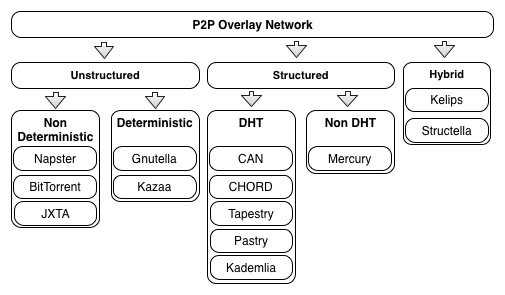
\includegraphics[width=\textwidth]{./img/p2porganizations.jpg}
  \end{center}
  \caption{Different types of P2P Overlay networks organizations}
  \label{fig:Different types of P2P Overlay networks organizations}
\end{figure}


\paragraph{\textbf{Unstructured -}} % (fold)
\label{par:Unstructured}

We call `Unstructured' to a P2P system that doesn't require or define any constraint for the placement of data, these include Napster, Kazaa and Gnutella, famous for it's file sharing capabilities, where nodes can share their local files directly, without storing the file in any specific Node. There is however a `caveat' in the Unstructured networks, by not having an inherent way of indexing the data present in the network, performing a lookup results of the cost of asking several nodes the whereabouts of a specific file or chunk of the file, creating a huge performance impact with an increasing number of nodes. In order to overcome this, Unstructured P2P networks offer several degrees of decentralization, one example is the evolution from Gnutella 0.4\cite{Definition2003} to Gnutella 0.6 \cite{T.Klingberg2002}\cite{Ripeanu2002a}, which added the concept of super nodes, entities responsible for storing the lookup tables for the files in parts of the network they are responsible for, increasing the performance, but adding centralized, single points of failure. 
\cite{Ranjan2006} classifies Unstructured networks into two types: deterministic and non-deterministic, defining that in a deterministic system, we can calculate before hand the number of hops needed to perform a lookup, knowing the predefined bounds, this includes systems such as Napster and BitTorrent\cite{Cohen2009}, in which the file transfers are decentralized, the object lookup remains centralized, keeping the data for the lookup tables stored in one place, which can be gathered by one of two ways : (i) peers inform directly the index server the files they have; or (ii) the index server performs a crawling in the network, just like a common web search engine, this gives this network a complexity of O(1) to perform a search, however systems like Gnutella 0.6, which added the super node concept, remain non deterministic because it's required to execute a query flood across all the super nodes to perform the search.

% paragraph Unstructured and Non-Deterministic (end)


\paragraph{\textbf{Structured with Distributed Hash Tables -}} % (fold)
\label{par:Structured with Distributed Hash Tables}
%CAN ;CHORD ;TAPESTRY; PASTRY; Kademlia




 % Peers in DHTs such as Chord, CAN, Pastry and Tapestry maintain an index for O(log (n)) peers where n is the total number of peers in the system. Inherent to the design of a DHT are the following issues [11]: (i) generation of node-ids and object-ids, called keys, using cryptographic/randomizing hash functions such as SHA- 1 [10, 66, 87]. The objects and nodes are mapped on the overlay network depending on their key value. Each node is assigned responsibility for managing a small number of objects; (ii) building up routing information (routing tables) at various nodes in the network. Each node maintains the network location information of a few other nodes in the network; and (iii) an efficient look-up query resolution scheme. Whenever a node in the overlay receives a look-up request, it must be able to resolve it within acceptable bounds such as in O(log (n)) time. This is achieved by routing the look-up request to the nodes in the network that are most likely to store the information about the desired object. Such probable nodes are identified by using the routing table entries. Though at the core various DHTs (Chord, CAN, Pastry etc.) are similar, still there exists substantial differences in the actual implementation of algorithms including the overlay network construction (network graph structure), routing table maintenance and node join/leave handling. The performance metrics for evaluating a DHT include fault-tolerance, load-balancing, efficiency of lookups and inserts and proximity awareness [73, 91]. In Table-3, we present the comparative analysis of Chord, Pastry, CAN and Tapestry based on basic performance and organisation parameters. Comprehensive details about the performance of some common DHTs under churn can be found in [70].
% Other classes of structured systems such as Mercury do not apply randomising hash functions for organising data
% items and nodes. 








% paragraph Structured with Distributed Hash Tables (end)

\paragraph{\textbf{Structured without Non-Distributed Hash Tables -}} % (fold)
\label{par:Structured without Non-Distributed Hash Tables}
%Mercury


% The Mercury system organises nodes into a circular overlay and places data contiguously on this ring. As Mercury does not apply hash functions, data partitioning among nodes is non-uniform. Hence it requires an explicit load-balancing scheme. 


% paragraph Structured without Non-Distributed Hash Tables (end)


% EXPLICAR AQUI QUE PODEMOS VER O SUMMARIO EM BAIXO :)

\begin{table}
  \begin{tabular}{| p{1.3cm} | p{1.9cm} | p{2cm} | p{2.5cm} | p{1.6cm} | p{1.8cm} | p{1.8cm} |}
    \hline                        
    \textbf{P2P system} & \textbf{Overlay Structure} & \textbf{Lookup Protocol} & \textbf{Networking parameter} & \textbf{Routing table size} & \textbf{Ruting complexity} & \textbf{Join/leave overhead} \\
    
    \hline
    Chord & 1 dimension, Hash ring & Matching key and NodeID & n= number of nodes in the network & O(log(n)) & O(log(n)) & O(log(n)\textsuperscript{2}) \\
    
    \hline
    Pastry & Plaxton style mesh structure & Matching key and prefix in NodeID & n\= number of nodes in the network, b\=base of identifier & O(log\textsubscript{b} (n)) & O(b log \textsubscript{b} (n)+b) & O(log(n)) \\
    
    \hline
    CAN & d-dimensional ID Space & Key value pair map to a point P in the D-dimensional space & n= number of nodes in the network, d=number of dimensions & O(2d) & O(d n\textsuperscript{1/2}) & O(2d) \\
    
    \hline
    Tapestry & Plaxton style mesh structure & Matching suffix in NodeID & n=number of nodes in the network, b=base of the identifier & O(log\textsubscript{b}(n)) & O(b log \textsubscript{b} (n)+b) & O(log(n)) \\
    \hline  
    
  \end{tabular}
  \caption{Summary of complexity of structured P2P systems}
  \label{tbl:Complexity of structured P2P systems}
\end{table}




\paragraph{\textbf{Hybrid -}} % (fold)
\label{par:Hybrid}
%Structella , Kelips



% In recent developments, new generation P2P systems have evolved to combine both unstructured and structured P2P networks. We refer to this class of systems as hybrid. Structella [27] is one such P2P system that replaces the random graph model of an unstructured overlay (Gnutella) with a structured overlay, while still adopting the search and content placement mechanism of unstructured overlays to support complex queries. Other hybrid P2P design includes Kelips [60] and its variants. Nodes in Kelips overlay periodically gossip to discover new members of the network, and during this process nodes may also learn about other nodes as a result of lookup
% 12
% communication. Other variant of Kelips [56] allows routing table entries to store information for every other node in the system. However, this approach is based on assumption that system experiences low churn rate [70]. Gossiping and one-hop routing approach has been used for maintaining the routing overlay in the work [108]. In Table 4, we summarize the different P2P routing substrate that are utilized by the existing algorithms for organizing a GRIS.


% paragraph Hybrid (end)



\subsubsection{3.2.4 Assurance and Trust}
% Fault tolerance
% Threshold Cryptography
% Reputation Management
% Economic Models




% 
%---------{Resource sharing using the Web as platform}------------
% 
\subsection{Resource sharing using the Web as platform} 
% Changed in the web Platform


\subsubsection{3.3.X What has been happening}
%Javascript
%WebRTC
%HTTP 2.0

\subsubsection{3.3.X Previous attempts}
%Merelo and friends





% ^^^^^^^^^^^^^^^^^^^^^^^^^^^^^^^^^^^^^^^^^^^^^^^^^^^^^^^^^^^^^^
% ~~~~~~~~~~~~~~~~~~~~~~~~~~~~~~~~~~~~~~~~~~~~~~~~~~~~~~~~~~~~~~
% ______________________________________________________________

% 
% Architecture
% 

\section{Architecture}

\subsection{Node Level}

\subsection{Client API}

\subsection{Storage}

\subsection{Reputation Mechanism}

\subsection{Job Scheduling}




% ^^^^^^^^^^^^^^^^^^^^^^^^^^^^^^^^^^^^^^^^^^^^^^^^^^^^^^^^^^^^^^
% ~~~~~~~~~~~~~~~~~~~~~~~~~~~~~~~~~~~~~~~~~~~~~~~~~~~~~~~~~~~~~~
% ______________________________________________________________

% 
% Evaluation
% 

\section{Evaluation}

\subsection{Lorem ipsum}

\subsubsection{Excepteur sint}



% ^^^^^^^^^^^^^^^^^^^^^^^^^^^^^^^^^^^^^^^^^^^^^^^^^^^^^^^^^^^^^^
% ~~~~~~~~~~~~~~~~~~~~~~~~~~~~~~~~~~~~~~~~~~~~~~~~~~~~~~~~~~~~~~
% ______________________________________________________________

% 
% Conclusions
% 

\section{Conclusions}

\subsection{Lorem ipsum}

\subsubsection{Excepteur sint}












% ^^^^^^^^^^^^^^^^^^^^^^^^^^^^^^^^^^^^^^^^^^^^^^^^^^^^^^^^^^^^^^
% ~~~~~~~~~~~~~~~~~~~~~~~~~~~~~~~~~~~~~~~~~~~~~~~~~~~~~~~~~~~~~~
% ______________________________________________________________


% 
% Acronym List
% 

% \acro{abc}[short version]{full version}
% \acro{efd}[shortAAA version]{full AAAversion}


% ^^^^^^^^^^^^^^^^^^^^^^^^^^^^^^^^^^^^^^^^^^^^^^^^^^^^^^^^^^^^^^
% ~~~~~~~~~~~~~~~~~~~~~~~~~~~~~~~~~~~~~~~~~~~~~~~~~~~~~~~~~~~~~~
% ______________________________________________________________

% 
% Bibliography
% 

\bibliographystyle{plain} 
\bibliography{/Users/DavidDias/Documents/bibtex/THESISREAD.bib}
\end{document}



% HOW TO CITE \cite{Ranjan2006}
% \section{sdasdasd}
% batatas sds \cite{Ranjan2006}
% asdada \cite{Afify}
% % \nocite{*}
% \cite{Merelo2007}


